\documentclass[12pt, a4paper]{article}
\title{Explaining the quantum algorithm for phase estimation using data structures}
%\date{January 1, 2020}
\author{Shashvat Shukla}


\usepackage{amsmath}
\usepackage{amsfonts}
\usepackage{amssymb}
\usepackage{physics}
\usepackage{mathtools}
\usepackage{verbatim}


\usepackage{graphicx}

\usepackage[amsthm, framed]{ntheorem}

\usepackage[colorlinks,citecolor=blue,urlcolor=blue,bookmarks=false,hypertexnames=true]{hyperref} 

%\usepackage{amsmath}
\DeclareMathOperator*{\argmax}{arg\,max}
\DeclareMathOperator*{\argmin}{arg\,min}

%\usepackage{mathtools}
\DeclarePairedDelimiter\ceil{\lceil}{\rceil}
\DeclarePairedDelimiter\floor{\lfloor}{\rfloor}
%\DeclarePairedDelimiter{\abs}{\lvert}{\rvert}

%\usepackage[amsthm, framed]{ntheorem}
\newtheorem{theorem}{Theorem}
\newtheorem{definition}{Definition}
\newtheorem{proposition}{Proposition}
\newtheorem{insight}{Insight}
\newtheorem*{problem*}{Problem}

% Complexity theory
\newcommand\bigO[1]{\mathcal{O}(#1)}


\begin{document}
	
	\maketitle
	
	\begin{abstract}
		The phase estimation algorithm is an algorithm for quantum computers that will be useful in physical simulation tasks and as a subroutine in Shor's quantum algorithm for prime factorisation. 
		Most textbook presentations of the phase estimation algorithm are driven by algebraic manipulation and prioritise details of how the quantum circuit acts while obscuring the algorithmic ideas.
		This paper explains the phase estimation algorithm in a new way, using elementary polynomial data structures from computer science as helpful high-level concepts. 
		Once the polynomial data structure concepts have been understood, the explanation of phase estimation can be stated in just a few lines.
				%This explanation involves two elementary data structures for storing polynomials: the \textit{coefficient} and \textit{point-value} representations. The quantum circuit for Fourier transform is motivated entirely from these two data structures as the efficient operation that converts between them.  . 
		%Our explanation of QPE uses high-level concepts and has minimal reliance on algebraic derivation. Once the polynomial data structure concepts have been understood, the explanation of QPE can be stated in just a few lines. As quantum information science continues to grow in popularity, we hope that this explanation will give educators an option for presenting higher level algorithm idea first, and leaving the algebraic manipulation to later or as an exercise.
	\end{abstract}

	\section{Introduction}
	
	\section{Quantum Phase Estimation}
	\label{sec:qpe}
	% Problem and set up
	
	\subsection{Setup}
	The Quantum Phase Estimation algorithm solves the following problem: Given a quantum state $\ket{\psi}$, and unitary $U$ and such that $\ket{\psi}$ is an eigenvector of $U$, find the corresponding eigenvalue. $\ket{\psi}$ is given as one copy of a quantum state, and the access to $U$ is given as access to black-box calls to a generalised controlled-$U$ gate. 
	
	We define the qudit-controlled-$U^d$ gate, as the gate that acts in the following manner:
	$(C_dU^d) \ket{j}\ket{\phi} = \ket{j}U^j\ket{\phi}$. This is a generalisation of the standard controlled-$U$ gate, which either applies the $U$ gate 0 or 1 times, depending on the controlling register. The qudit-controlled-$U^d$ gate applies the $U$ gate $j$ times, if the number in the controlling register is $j$. 
	
	The Quantum Phase Estimation algorithm is a quantum circuit that uses the qudit-controlled-$U^d$ gates and the quantum state $\ket{\psi}$ to determine the eigenvalue. 
	
	Say $U \ket{\psi} = e^{i 2 \pi r} \ket{\psi}$. We can specify the bits of precision used in our algorithm as a parameter $n$ (and define $N = 2^n$) such that $r \approx \frac{k}{N}$ where $k\in \mathbb{N}$. Let $\omega_N = e^{i 2 \pi /N}$, the principal $N$-th root of unity. Thus our goal is to determine $k$ s.t. $U \ket{\psi} \approx \omega^{k}_N \ket{\psi}$ (See Figure \ref{fig:approx}). 
\begin{figure}
	\centering
	\title{\textbf{\underline{Approximating eigenvalues by roots of unity}}}
	\includegraphics[width=0.7\linewidth]{approx}
	\caption{The goal of QPE is to find the eigenvalue of $U$ corresponding to $\ket{\psi}$. For a fixed precision $N$, QPE identifies the closest $N$-th root of unity to the true eigenvalue ($e^{i 2 \pi r}$). Thus we can see the goal of QPE as identifying the value $k$ such that $r$ is closest to $\frac{k}{N}$. Notice how increasing $N$ will make the algorithm more accurate as there will be a finer discretisation of the circle.}
	\label{fig:approx}
\end{figure}
	
	\subsection{Polynomial Data Structures}
	
	\begin{figure}
		\centering
		\title{\textbf{\underline{Polynomial Data Structures}}}
		
		\vspace{5mm}
		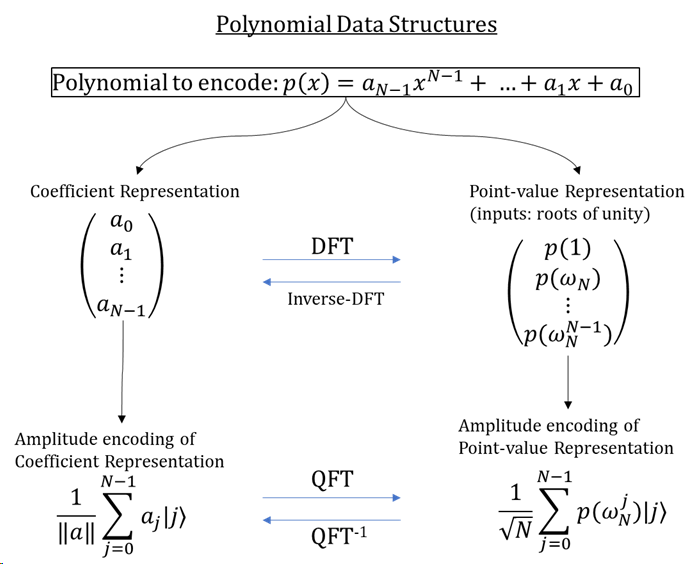
\includegraphics[width=\linewidth]{polyds.jpg}
		\caption{This figure depicts the two polynomial data structures and their quantum analogues whic are used in our explanation of QPE.}
		\label{fig:polyds}
	\end{figure}
	
	
	
	This subsection introduces the key data structure concepts that we use in our explanation of QPE. Figure \ref{fig:polyds} shows these concepts and how they are related in one graphic. Once the concepts in this subsection have been understood, then QPE can be explained in just a few lines as we do in the next subsection.
	
	The \underline{amplitude encoding of a vector} is the quantum state obtained from normalising the components of a vector and putting them into amplitudes of a quantum state, for example as: $v= [v_0 ... v_{N-1}] \rightarrow \frac{1}{\norm{v}} \sum_{i=0}^{N-1} v_i \ket{i}$.
	
	%rewrite this one carefully
	The \underline{coefficient representation of a polynomial} is a vector containing all its coefficients. For example $p(x) = a_{N-1}x^{N-1} + ... + a_0$ is represented as $a = [a_0 ... a_{N-1}]$. The final step of QPE involves the \textit{amplitude encoding} of the coefficient representation of a polynomial so $p(x) = a_{N-1}x^{N-1} + ... + a_0$ is stored as $\frac{1}{\norm{a}} \sum_{i=0}^{N-1} a_i \ket{i}$. Since the polynomial in question turns out to be a single term polynomial $x^k$, the amplitude encoding of it is just $\ket{k}$. 
	
	The \underline{point-value representation of a polynomial} is motivated by the fact that a polynomial ($p$ with degree less than $N$) is represented by a series of points $\{(x_0,p(x_0)), ..., (x_{N-1},p(x_{N-1}))\}$. For example, with two points, we represent the unique line that passes through those points. If we fix the inputs $\{x_0, ..., x_{N-1}\}$ at which we will evaluate the polynomial, then we can just store the values $[p(x_0)...p(x_{N-1})]$ as a vector. We can choose any set of $N$ input values. For our purposes we will choose the N-th roots of unity $\{1,\omega_N, ..., \omega_N^{N-1}\}$ as our set of inputs and store $[p(1)...p(\omega_N^{N-1})]$. This choice makes it efficient to convert between the coefficient and point-value representations. 
	
	Consider how we can convert from the coefficient representation to the point value representation. We have to evaluate the polynomial at each of the $N$ inputs. Converting $[1,\omega_N, ..., \omega_N^{N-1}]$ to  $[p(1),...,p(\omega_N^{N-1})]$ requires the following transformation:

	$$p(\omega_N^l) = \sum_{j=0}^{N-1} a_j \omega_N^{jl} = \sum_{j=0}^{N-1} a_j e^{i2\pi jl/N},$$
	
	which is exactly the Discrete Fourier Transform. 
	
	%We illustrate this in Figure \ref{fig:dft}.
	
	When normalised by a $\frac{1}{\sqrt{N}}$ factor, the Discrete Fourier Transform is a unitary matrix. If we implement this matrix as a quantum circuit, it converts from the \textit{amplitude encoding} of the coefficient representation to the \textit{amplitude encoding} of the point-value representation. This circuit is called the Quantum Fourier Transform and it can be implemented efficiently due to a divide-and-conquer algorithm. The details of this are interesting but not essential for a first understanding of QPE, so we discuss it in the next section.
	
	The second step of the QPE algorithm performs an inverse-QFT to convert from the amplitude encoding of the point-value representation to the amplitude encoding of the coefficient representation.
	
	\subsection{Algorithm}
	
	\begin{figure}
		\centering
		\title{\textbf{\underline{Quantum Phase Estimation Algorithm}}}
		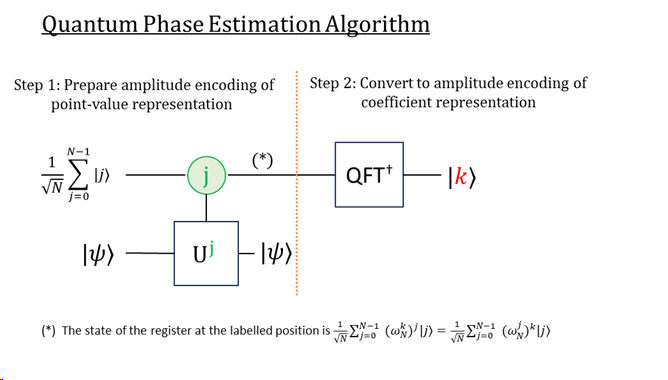
\includegraphics{qpe_algorithm.jpg}
		\caption{High level circuit explaining the Quantum Phase Estimation Algorithm. The algorithm has two steps. Step 1 prepares $\frac{1}{\sqrt{N}}\sum_{j=0}^{N-1}  (\omega^{k}_N)^j \ket{j} = \frac{1}{\sqrt{N}}\sum_{j=0}^{N-1}  (\omega^{j}_N)^k \ket{j}$, which is the amplitude encoding of the point-value representation of the polynomial $x^k$. Step 2 converts to the amplitude encoding of the coefficient representation, yielding $k$.}
		\label{fig:qpealgorithm}
	\end{figure}
	
	
	This circuit has two parts. The first part \textbf{prepares an amplitude encoding of the point-value representation of the polynomial} $\bf{x^k}$. This can be shown from a simple derivation, notice that the resultant state has amplitudes equal to taking each root of unity to the $k$-th power: 
	\begin{align*}
		&C_dU^d [\frac{1}{\sqrt{N}}\sum_{j=0}^{N-1} \ket{j}\ket{\psi}] \\
		&=\frac{1}{\sqrt{N}}\sum_{j=0}^{N-1}  (\omega^{k}_N)^j \ket{j} \ket{\psi}  &&(\text{Since } U\ket{\psi} = \omega_N^k \ket{\psi})\\
		&=\frac{1}{\sqrt{N}}\sum_{j=0}^{N-1}  (\omega^{j}_N)^k \ket{j} \ket{\psi} \\
	\end{align*}
	
	The second part \textbf{converts to the amplitude encoding of the coefficient representation of the polynomial} using the inverse-QFT, giving us the outcome $\ket{k}$ since the polynomial was $x^k$. 
	
	%\section{Quantum Fourier Transform}
	
	%uses the inverse-QFT (which is the inverse-DFT on the amplitudes), 
	%The high-level concepts mentioned in bold in this section are explained in the next subsection. 
	 
	%One last paragraph on how DFT converts 
	
	
	%Polynomials can be stored in classical computers as vectors of coefficients (coefficient representation), or else by simply evaluating the polynomial at a sufficient number of points (point-value representation). In the latter case, we need to evaluate the polynomial at enough points such that the polynomial can be uniquely identified from the points (for example storing two points is enough to uniquely identify a linear function, three points is enough for a quadratic function, etc.). These data structures have different strengths so we want to be able to efficiently convert between them. In particular, choosing to evaluate the polynomial at a set of roots of unity makes this efficient, and this transformation is called the Discrete Fourier Transform. 
	
	%Naive algorithms for this conversion take $O(n^2)$ time, but if the points at which the polynomial is evaluated are chosen to be the roots of unity, then it can be done more efficiently. This transformation is called the Discrete Fourier Transform, and it can be implemented in $O(n \log n)$ time using a divide-and-conquer algorithm called the Fast Fourier Transform algorithm. 
	

	
	
	
	\begin{comment}

	
	\section{Polynomial Data Structures}
	
	This section introduces some background on polynomial data structures, which we will use in our explanation of QPE.
	
	\subsection{The coefficient and point-value representations}
	Polynomials are functions of the form 
	\begin{equation}
	f(x) = a_{n-1} x^{n-1} + ... + a_1 x + a_0.
	\end{equation}
	A natural way to store polynomials in classical computers is thus the \textit{coefficient} representation, i.e. storing $(a_{n-1}, ... ,a_0)$ as a vector. We can choose any sufficiently large $n$ as the size of our vector, which we call the degree-bound (as the degree is \textbf{less} than this number).  Storing polynomials this way gives us familiar algorithms for operating with the polynomials.
	\begin{itemize}
		\item \textbf{Addition:} To add two polynomials, we simply add the two coefficient vectors. This takes $O(n)$ time.
		\item \textbf{Evaluation:} We can evaluate the polynomial on a given input in $O(n)$ time. To do this one has to just avoid computing each power of $x$ independently, as this wastes multiplication operations. One famous trick to achieve this is Horner's rule. 
		\item \textbf{Multiplication:} We can multiply polynomials in $O(n^2)$ time, by means of the familiar long-multiplication algorithm. That is, we would perform the multiplication by the distributive law and collect like-power terms together. As multiplication increases the degree of polynomials, one should check that the resultant polynomial is still degree-bound $n$, but if not, a new vector of appropriate size should be used. 
	\end{itemize}
	   
	The \textit{point-value} representation of polynomials is an alternative data structure that can multiply polynomials in $O(n)$ time. Instead of storing the coefficients, we store the polynomial evaluated at any $n$ inputs of our choosing. For example instead of storing the vector $(1,2,-1,1)$ for $p(x) = x^3 + 2x^2 - x + 1$, we store $(p(0),p(1),p(-1),p(2)) = (1,3,3,15)$.
	
	Once these inputs are chosen, this representation associates a unique vector to each polynomial, because given $n$ points there is a unique degree-bound $n$ polynomial that passes through all those points. For example, given three points on a plane there is either a quadratic function or a line that passes through all three of them. This is because $n$ points give us a system of $n$ linear equations to solve for at most $n$ coefficients of the polynomial. 
	
	In this representation, we can both add and multiply in $O(n)$ time, simply by doing a component-wise addition or multiplication, because $(pq)(x_i) = p(x_i) q(x_i)$. This remains a unique encoding of some polynomial so long as the degree of the resultant polynomial is still less than the degree-bound. 
	
	The trade-off here is that the point-value representation cannot evaluate the polynomial on arbitrary inputs in any straightforward way. 
	
	\subsection{Converting between representations}
	One way to evaluate the polynomial on a given input, we would be able to evaluate the polynomial on arbitrary inputs by converting back to the coefficient representation. 
	
	
	This conversion can be done in $O(n\log n)$ time if we choose a very special set of points, namely the $n$-th roots of unity. 
	
	\section{Quantum Phase Estimation}
	
	Quantum Phase Estimation solves the following computational task:
	\begin{problem*}
		Let $N\in \mathbb{Z}$,$U$ be a unitary, and $\ket{\psi}$ be a quantum state such that $U\ket{\psi} = \omega^k_N \ket{\psi}$ (i.e. $\ket{\psi}$ is an eigenvector of $U$ with eigenvalue that is some $N$-th root of unity.). You are given access to $C_jU^j = \sum_{j=0}^{N-1} \ket{j}\bra{j} \otimes U^j$ gate. Find $k$. 
		\end{problem*}
	
	The Quantum Phase Estimation algorithm has two steps:
	\begin{enumerate}
		\item Prepare the point-value representation of $x^k$, using the $N$-th roots of unity as inputs: 
		
		Perform \begin{align*}
			&C_jU^j [(\frac{1}{\sqrt{N}}\sum_{j=0}^{N-1} \ket{j})\otimes\ket{\psi}] \\
			&=\frac{1}{\sqrt{N}}\sum_{j=0}^{N-1} C_jU^j (\ket{j}\otimes\ket{\psi}) \\
			&=\frac{1}{\sqrt{N}}\sum_{j=0}^{N-1}  (\ket{j}\otimes (\omega^{k}_N)^j\ket{\psi}) \\
			&\underset{\text{(i)}}{=}[\frac{1}{\sqrt{N}}\sum_{j=0}^{N-1}  (\omega^{k}_N)^j \ket{j}]\otimes \ket{\psi} \\
			&\underset{\text{(ii)}}{=}[\frac{1}{\sqrt{N}}\sum_{j=0}^{N-1}  (\omega^{j}_N)^k \ket{j}]\otimes \ket{\psi} \\
		\end{align*}
		The step labelled (i) is simply the moving of constants from one register to the other, and is called ``phase kickback'' as it seems surprising that a phase we think we are applying on $\ket{\psi}$ actually gets applied on the controlling register. In fact, this is only a surprise because of the way we commonly interpret controlled gates, i.e. as being controlled by a controlled register and acting only on the target register. In reality, controlled gates are also two-register interactions and act on the whole system. 
		The step labelled (ii) is the only non-trivial part of our derivation. 
		\item Convert to the coefficient representation to obtain $k$. That is, use the inverse-QFT and measure to obtain $k$. 
		$$ QFT^{\dagger}[\frac{1}{\sqrt{N}}\sum_{j=0}^{N-1}  (\omega^{j}_N)^k \ket{j}] = \ket{k}$$
	\end{enumerate}
	
	
	\end{comment}
	
	
	%\section{Beyond QPE}
	
	%\subsection{QPE with approximation error}
	
	%In the explanation of QPE in section \ref{sec:qpe}, I assumed that we raised the precision $n$ high enough so that the eigenvalue was an $N-th$ ($N=2^n$)root of unity, and the QPE was exact. Can polynomial data structures explain the behaviour of QPE when it is not exact? 
	
	
	
	%\section{Other algorithms from a data structure perspective}
	
	% Deutsch- Jozsa is about making either the uniform superposition state, or a state perpendicular to that , depending on which oracle you have gotten
	
	% The forrelation problem is just about taking that inner product
	
	% Simon's algorithm is about preparing a state that is a superposition of j such that j . s = 0
	% This is a great example of a more complicated procedure of extracting information from a state, but still using the quantum algorithm to make that state. Quantum algorithm gets you some way and sampling gets you the rest of the way. Grover's is also like that in a sense. 
	
	% HHL is the most obviously data structure related algorithm 
	
	% Shor's is about QPE and the coset representation of integers 
	
	% I think Bernstein Vazirani is some kind of Forrelation idea 
	\section{Notes}
	This explanation was motivated by reading Ref. \cite{cormen2009algorithms_ch30}.
	
	% I perceived the traditional explanations to leave the mechanism of the algorithm up to a computation. It would be left to a "computation by the reader", that the probability of measuring certain outcomes was 0 and hence any outcome is one of the desirable ones. This would mean that circuits were merely stated and could be checked to work by means of computation, but no motivation or explanation was given that might aid in memory or in coming up with new algorithms for oneself. 
	
	
	% A story about QFT and AHSP can be told that sees QFT as mapping from group elements to characters 
	% See https://courses.cs.washington.edu/courses/cse490q/20au/lectures/27-hsp.pdf 

	\bibliographystyle{ieeetr}
	
	\bibliography{References}

	
\end{document}